\documentclass{article}


\usepackage[utf8]{inputenc} % Поддержка UTF-8
\usepackage[russian]{babel} % Поддержка русского языка
\usepackage{amsmath, amsfonts, amssymb} % Для математических выражений и символов
\usepackage{geometry} % Настройка полей страницы
\geometry{top=2cm, bottom=2cm, left=2.5cm, right=2.5cm}
\usepackage{enumitem} % Списки с кастомными настройками
\usepackage{hyperref} % Для гиперссылок
\usepackage{graphicx}
\usepackage{hyperref}

\title{Theory of linear models}
\author{Sharabarin Mikhail}
\date{18.02.2025}

\begin{document}
\section{Theory}
\subsection{Singular decomposition}
\href{https://www.geeksforgeeks.org/singular-value-decomposition-svd/}{\textbf{Singular value decomposition}} -- method in linear algebra used to decompose
    matrix in three different matrices, making it easier to analyze and manipulate.


\begin{figure}[h]     \centering     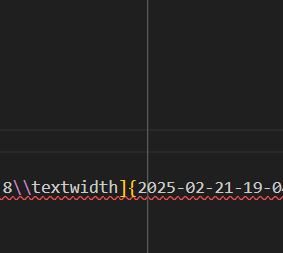
\includegraphics[width=0.5\textwidth]{2025-02-21-19-05-35.png}     \caption{Caption for }     \label{} \end{figure}



\end{document}